\section{Moment of Inertia}

%Lecture 33
\textit{Note that in statics we are using the second moment of area as our moment of inertia. In dynamics a different moment of inertia is used (the mass moment of inertia). The differences between these two quantities are summarized in the table below: }

\begin{table}[]
\centering
\begin{tabular}{c|c|c}
 & \textbf{Mass moment of inertia} & \textbf{Area moment of inertia} \\ \hline
\textbf{Other names} &  & Second moment of area \\
 &  &  \\
\textbf{Description} & \begin{tabular}[c]{@{}c@{}}Determines the torque \\ needed to produce a \\ desired angular rotation \\ about an axis of rotation \\ (resistance to rotation)\end{tabular} & \begin{tabular}[c]{@{}c@{}}Determines the moment \\ needed to produce a \\ desired curvature \\ about an axis \\ (resistance to bending)\end{tabular} \\
 &  &  \\
\textbf{Equations} & 
\begin{tabular}[c]{@{}c@{}} 
 \[I_{P,\hat{a}} = \iiint_\mathcal{B} \rho r^2 \,dV\] \\ 
 \end{tabular} &

 \begin{tabular}[c]{@{}c@{}}
 \[I_x = \int_{A}^{} y^2 \,dA \]\\ 
 \[I_y = \int_{A}^{} x^2 \,dA \]\\ 
 \[J_O = \int_{A}^{} r^2 \,dA = \int_{A}^{} (x^2+y^2) \,dA\]
 \end{tabular} \\
 
 &  \\
\textbf{Units} & length*mass\textasciicircum{}2 & length\textasciicircum{}4 \\
 &  &  \\
\textbf{Typical Equations} & \[\tau = I\alpha \] &  \[\sigma = (My)/I \]\\
 &  &  \\
\textbf{Courses} & TAM 212 & TAM 210, TAM 251
\end{tabular}
\end{table}

\subsection{Moment of Inertia (Second Moment of Area)}

The moment of inertia used in statics is the "second moment of area", which is a mass property that determines the amount of torque that is needed to create an angular acceleration about a specific axis of rotation. The dimension of the area moment of inertia is $length^4$.\\

Moment of inertia about the x-axis:  \[I_x = \int_{A}^{} y^2 \,dA \]

Moment of inertia about the y-axis: \[I_y = \int_{A}^{} x^2 \,dA \]

Polar moment of inertia: \[J_O = \int_{A}^{} r^2 \,dA = \int_{A}^{} (x^2+y^2) \,dA\]
\textit{Note that the polar moment of inertia depicts the measure of the distribution of area about a point (usually the origin), rather than about an axis.}

\subsection{Parallel axis theorum}

\blue{Need to transcribe this to be the correct format and drawings}

\begin{figure*}[!h]
\centering
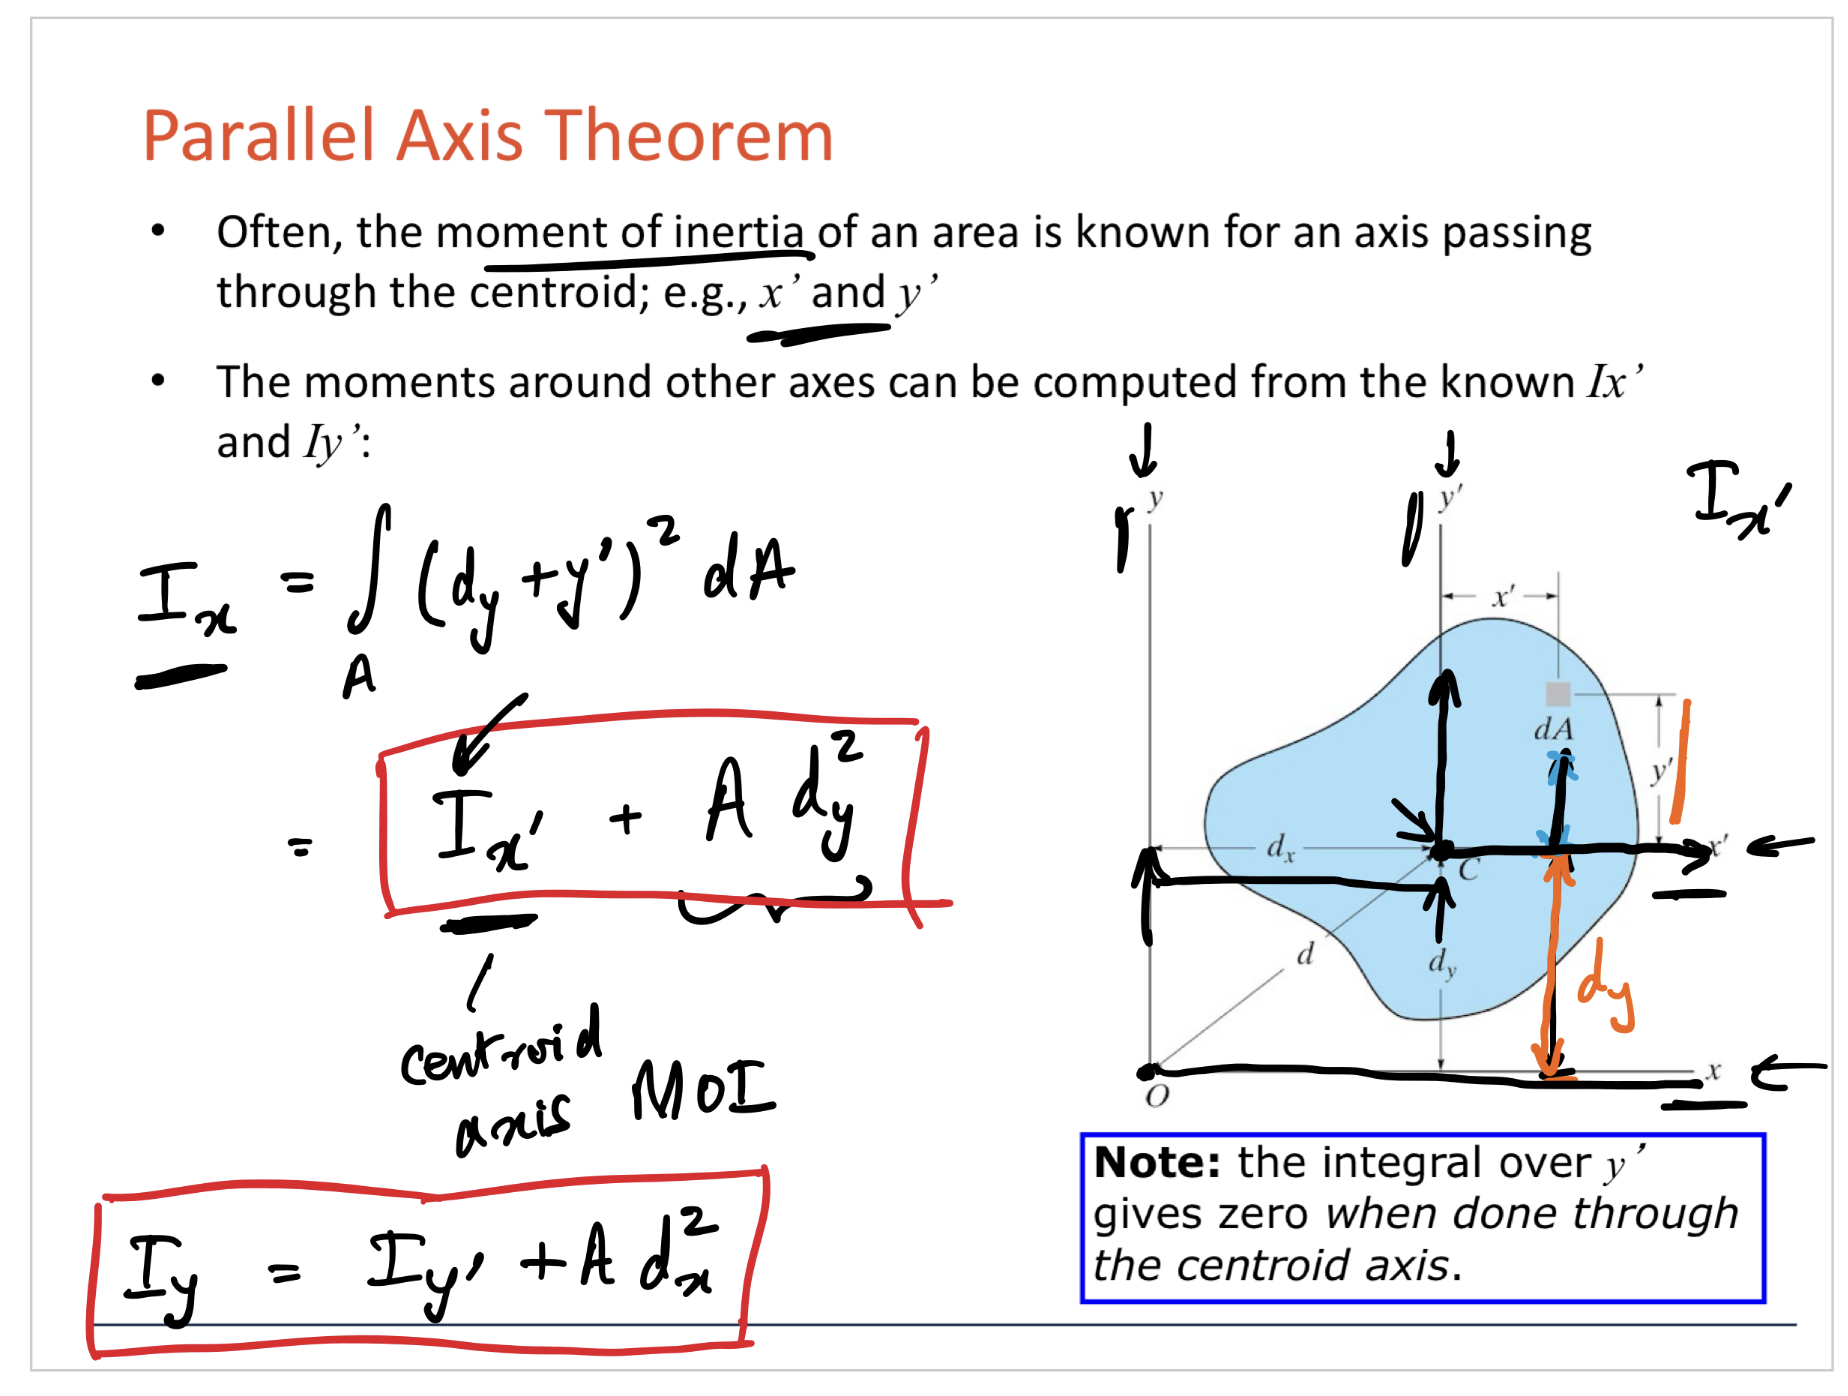
\includegraphics[angle=0, width=\textwidth]{MOIFigures/ParallelAxisThm.png}
\vspace{-2mm}
\caption{\small \blue{Taken from TAM 210 Lecture 3 - Slide 3}}
\vspace{-3mm}
\label{Fig:ParallelAxisThm}
\end{figure*}


\subsection{Combining moments of inertia}

\blue{Need to transcribe this to be the correct format and drawings - show the example problem with the house-shaped object.}

\begin{figure*}[!h]
\centering
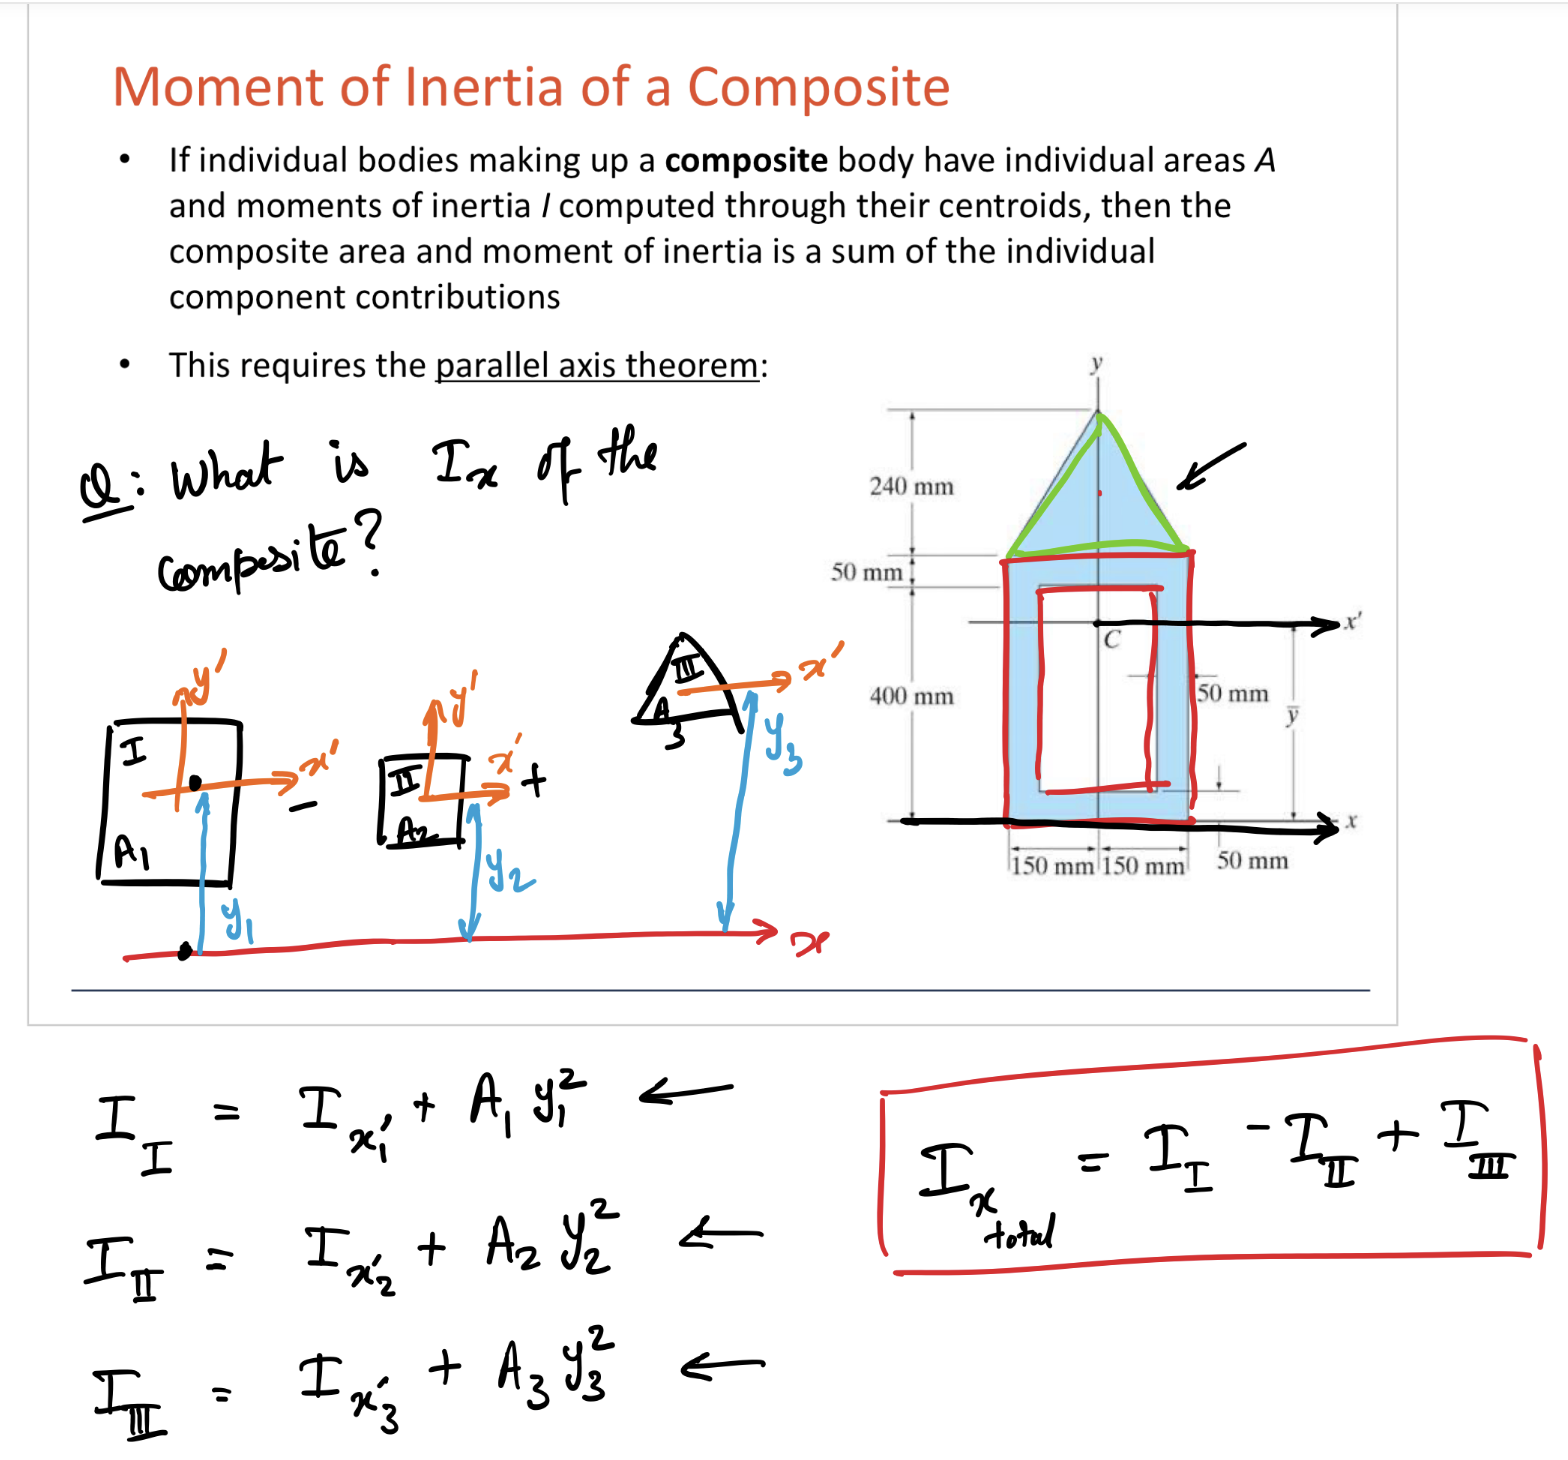
\includegraphics[angle=0, width=\textwidth]{MOIFigures/MOIComposite.png}
\vspace{-2mm}
\caption{\small \blue{Taken from TAM 210 Lecture 3 - Slide 3}}
\vspace{-3mm}
\label{Fig:MOIComposite}
\end{figure*}

\subsection{Moment of inertia for typical shapes}

\begin{figure*}[!h]
\centering
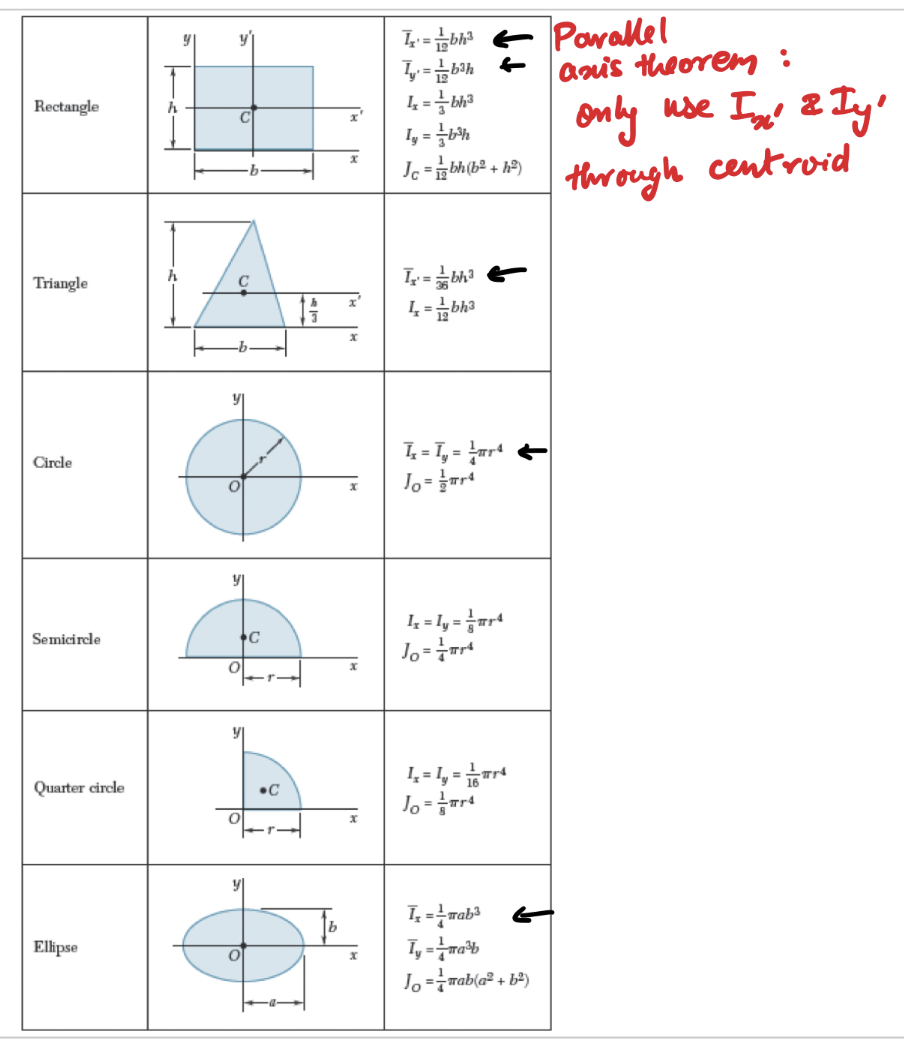
\includegraphics[angle=0, width=\textwidth]{MOIFigures/TypicalMOI.png}
\vspace{-2mm}
\caption{\small \blue{Taken from TAM 210 Lecture 3 - Slide 3}}
\vspace{-3mm}
\label{Fig:TypicalMOI}
\end{figure*}

